\documentclass[11pt]{article}
\usepackage[a4paper, margin=2cm]{geometry}
\usepackage[utf8]{inputenc}
\usepackage{babel}
\usepackage[spanish]{layout}
\usepackage[article]{ragged2e}
\usepackage{textcomp}
\usepackage{amsmath}
\usepackage{amssymb}
\usepackage{amsfonts}
\usepackage{proof}
\usepackage{enumerate}
\usepackage{graphicx}
\usepackage{multirow}
\usepackage{caption}
\usepackage{subcaption}

\setlength{\parindent}{0pt}

\title{
    Trabajo Práctico Lógica Borrosa \\
    \large Introducción a la Inteligencia Artificial}
\author{Mellino, Natalia \and Farizano, Juan Ignacio}

\date{}

\begin{document}
\maketitle

\noindent\rule{\textwidth}{1pt}

\section{Enunciado}

\subsection*{Introducción}
Nos interesa estudiar la \textbf{esperanza de vida} (en años) de una persona y cómo
influyen ciertos factores en ella. Los factores que influyen en ella son la \textbf{edad} actual,
el \textbf{nivel de estrés} que puede afectarle física y mentalmente,
el \textbf{nivel de actividad física} que realiza y el \textbf{nivel de salud}
que presenta actualmente.

\subsection*{Reglas}

\begin{enumerate}
    \item Si edad es \emph{persona mayor} entonces esperanza de vida es \emph{alta}.
    \item Si edad es \emph{niño}, nivel de salud es \emph{saludable} o \emph{muy saludable}, entonces esperanza es \emph{alta}.
    \item Si edad es \emph{niño}, nivel de salud es \emph{poco enfermo}, entonces esperanza es \emph{media}. 
    \item Si edad es \emph{niño}, nivel de salud es \emph{enfermo}, entonces esperanza es \emph{pobre}.
    \item Si edad es \emph{adulto}, nivel de estrés es \emph{bajo} o \emph{mediano} y nivel actividad física no es \emph{bajo} y nivel de salud no es \emph{enfermo}, entonces esperanza es \emph{alta}. 
    \item Si edad es \emph{adulto}, nivel de estrés es no \emph{bajo} y nivel actividad física es \emph{bajo} o \emph{mediano} y nivel de salud es \emph{enfermo} o \emph{poco enfermo}, entonces esperanza es \emph{media}.
    \item Si edad es \emph{adulto}, nivel de estrés es \emph{alto}, nivel de actividad física es \emph{bajo}, y nivel de salud es \emph{enfermo} o \emph{poco enfermo}, entonces esperanza es \emph{baja}.
    \item Si edad es \emph{joven} y nivel de salud es \emph{muy saludable} o \emph{saludable}, entonces esperanza es \emph{alta}. 
    \item Si edad es \emph{joven}, nivel de estrés es no \emph{alto}, nivel actividad física es no \emph{alto} y nivel de salud es no \emph{enfermo}, entonces esperanza es \emph{media}. 
    \item Si edad es \emph{joven}, nivel de estrés es \emph{mediano}, nivel actividad física es no \emph{alto} y nivel de salud es \emph{enfermo} o \emph{poco enfermo}, entonces esperanza es \emph{baja}.
    \item Si edad es joven, nivel de estrés es \emph{alto}, nivel actividad física es \emph{bajo} y nivel de salud es \emph{enfermo}, entonces esperanza es \emph{pobre}.
\end{enumerate}

\subsection*{Rangos}

\begin{itemize}
    \item Rango de Edad [0, 120]:
        \begin{itemize}
            \item Niño: función semitrapezoidal descendente que de 0 a 10 vale 1 y de 15 a 120 vale 0
            \item Joven: función sinoidal que en 14 vale 0, en 19 vale 1 y en 24 vale 0
            \item Adulto: función sinoidal que en 18 vale 0, en 41.5 vale 1 y en 65 vale 0
            \item Persona mayor: función semitrapezoidal ascendente que de 0 a 60 vale y de 70 a 120 vale 1
        \end{itemize}
    \item Rango de Nivel de estrés [0, 10]:
        \begin{itemize}
            \item Bajo: función semitrapezoidal descendente que de 0 a 3 vale 1 y de 4 a 10 vale 0
            \item Mediano: función triangular que de 0 a 3 vale 0, en 4.5 vale 1 y de 6 a 10 vale 0
            \item Alto: función semitrapezoidal ascendente que de 0 a 5.5 vale 0 y de 7.5 a 10 vale 1
        \end{itemize}
    \item Rango de Nivel de actividad física [0, 10]:
        \begin{itemize}
            \item Bajo: función semitrapezoidal descendente que en 0 vale 1 y de 4 a 10 vale 0.
            \item Mediano: función triangular que de 0 a 3 vale 0, en 5 vale 1 y de 7 a 10 vale 0.
            \item Alto: función semitrapezoidal ascendente que de 0 a 6 vale 0 y en 10 vale 1.
        \end{itemize}
    \item Rango de Nivel de salud [0, 10]:
        \begin{itemize}
            \item Enfermo: función semitrapezoidal descendente que en 0 vale 1 y de 3.3 a 10 vale 0.
            \item Poco enfermo: función triangular que en 0 vale 0, en 3.3 vale 1 y de 6.6 a 10 vale 0.
            \item Saludable: función triangular que de 0 a 3.3 vale 0, en 6.6 vale 1 y de 6.6 a 10 vale 0
            \item Muy saludable: función semitrapezoidal ascendente que de 0 a 6.6 vale 0 y en 10 vale 1
        \end{itemize}
    \item Rango de Esperanza de vida [0, 120]:
    \begin{itemize}
        \item Pobre: función semitrapezoidal descendente que de 0 a 10 vale 1 y de 20 a 120 vale 0
        \item Baja: función sinoidal que en 18 vale 0, en 34 vale 1 y en 50 vale 0
        \item Media: función sinoidal que en 45 vale 0, en 57.5 vale 1 y en 70 vale 0
        \item Alta: función semitrapezoidal ascendente que de 0 a 65 vale y de 80 a 120 vale 1
    \end{itemize}
\end{itemize}


\subsection*{Consignas}

\begin{enumerate}[a)]
    \item Distinguir las variables lingüísticas de entrada y salida.
    \item Determinar la esperanza de vida para una persona de 18 años, un nivel de estrés
          igual a 5, nivel de actividad física 4 y un nivel de salud 9. Interprete \\
    \textbf{Obs:} defuzzificar con el método de mean max. 
    \item Repita el punto anterior pero para una edad de 42, estrés de 5, nivel 3
          de actividad física y nivel 6 de salud.
    \item Indique qué reglas se dispararon en los items anteriores.
    \item Repetir los items c) y d) con una Edad de 90.
\end{enumerate}

\newpage

\section{Resolución}

\subsection*{Apartado a)}

\begin{itemize}
    \item \textbf{Variables de entrada}
        \begin{itemize}
            \item Edad
            \begin{figure}[h!]
                \begin{center}
                  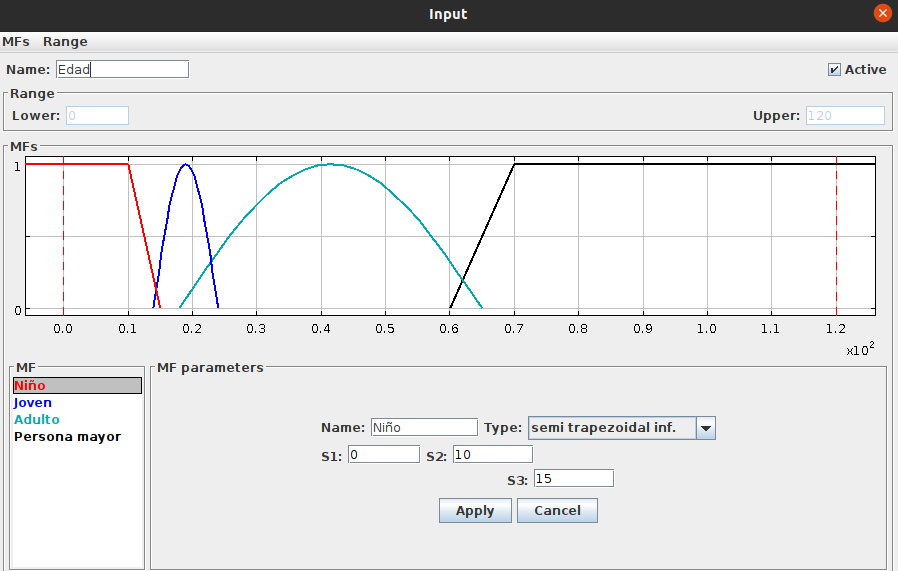
\includegraphics[width=0.6\linewidth]{edad.png}
                \end{center}
            \end{figure}
            \item Nivel de estrés
            \begin{figure}[h!]
                \begin{center}
                  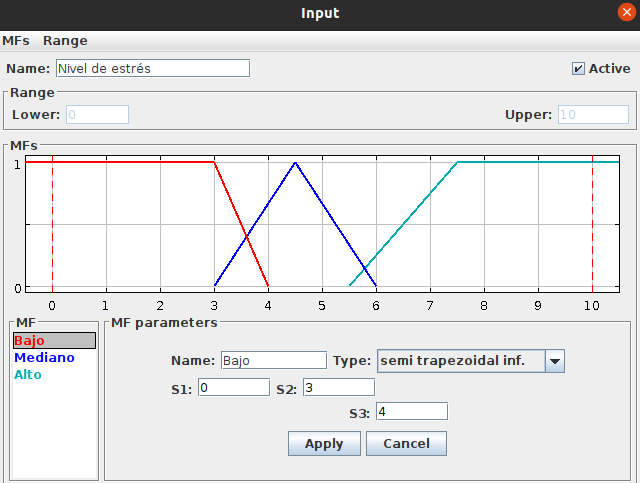
\includegraphics[width=0.6\linewidth]{estres.png}
                \end{center}
            \end{figure}
            \newpage
            \item Nivel de actividad física
            \begin{figure}[h!]
                \begin{center}
                  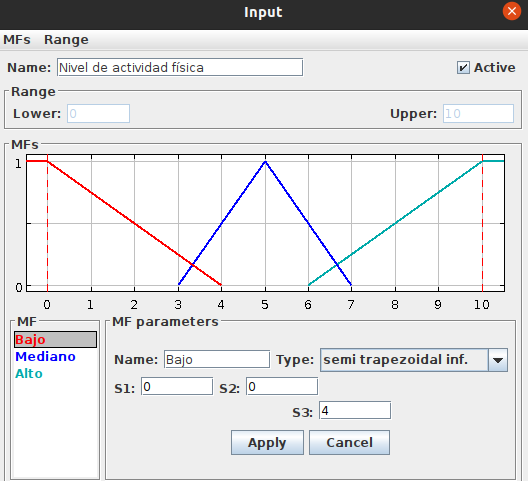
\includegraphics[width=0.6\linewidth]{actividad.png}
                \end{center}
            \end{figure}
            \item Nivel de salud
            \begin{figure}[h!]
                \begin{center}
                  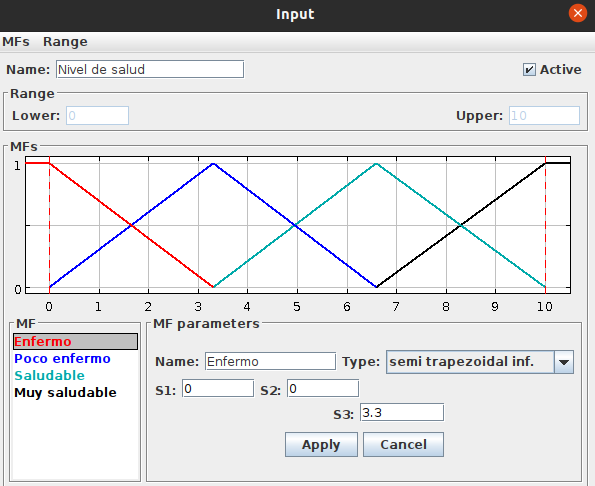
\includegraphics[width=0.6\linewidth]{salud.png}
                \end{center}
            \end{figure}
        \end{itemize}
    \newpage
    \item \textbf{Variables de salida}
        \begin{itemize}
            \item Esperanza de vida 
            \begin{figure}[h!]
                \begin{center}
                  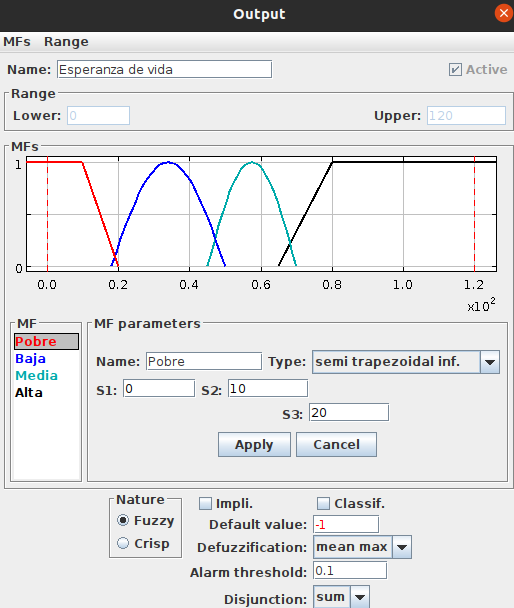
\includegraphics[width=0.6\linewidth]{esperanza.png}
                \end{center}
            \end{figure}
        \end{itemize}
\end{itemize}

\subsection*{Apartado b)}

La esperanza de vida estimada es de 100 años. Interpretamos que el individuo
sobre el que se realizó la prueba goza de buena calidad de vida por el momento. Las
reglas que se dispararon fueron las reglas 8 y 9 del enuciado.

\subsection*{Apartado c)}

La esperanza de vida estimada es de 57.5 años. De esto se interpreta que el individuo
posee actualmente una salud vulnerable y si no se cuida peligra su bienestar. La única
regla que se disparó fue la regla 6 del enunciado.
% 19 => 6

\subsection{Apartado d)}
Se encuentra resuelto en los apartados anteriores.

\subsection*{Apartado e)}
La esperanza de vida estimada es de 100 años Al ser ya una persona mayor, claramente
su esperanza de vida ya de por sí es elevada y podemos decir que el sujeto ha 
gozado de buena calidad de vida. La única regla disparada es la regla número 1
del enunciado.

\section{Conclusiones}

\begin{itemize}
    \item Nuestra principal dificultad se presentó al elegir el dominio, pasamos por 
          varias opciones pero se complicaba el modelarlos al no tener un conocimiento
          más profundo sobre ellos.
    \item Como los conjuntos borrosos elegidos no son fácilmente distinguibles,
          nos basamos en datos proporcionados por la OMS y modificados para 
          adaptarlos a nuestro modelo.
    \item Nuestra idea original involucraba dos variables de entrada adicionales, 
          pero esto complejizaba demasiado el proceso de crear reglas. Así que
          se opto por hacer un balance entre la moderación con la cantidad de reglas
          y seguir manteniendo un nivel mínimo de complejidad.
    \item La cantidad de variables elegida para el dominio hizo que nuestro abanico de 
          reglas posibles sea muy amplio. Nuestra principal dificultad consistió justamente 
          en tratar de reducir esas reglas lo máximo posible tratando de mantener
          un sistema de inferencias razonable.
    \item Al tener variedad de reglasde inferencia que utilizan los operadores \emph{or} y \emph{not}
          hemos tenido que separarlas en distintas reglas.
\end{itemize}

\end{document}
